\documentclass[10pt]{report}\usepackage[]{graphicx}\usepackage[]{xcolor}
% maxwidth is the original width if it is less than linewidth
% otherwise use linewidth (to make sure the graphics do not exceed the margin)
\makeatletter
\def\maxwidth{ %
  \ifdim\Gin@nat@width>\linewidth
    \linewidth
  \else
    \Gin@nat@width
  \fi
}
\makeatother

\definecolor{fgcolor}{rgb}{0.345, 0.345, 0.345}
\newcommand{\hlnum}[1]{\textcolor[rgb]{0.686,0.059,0.569}{#1}}%
\newcommand{\hlstr}[1]{\textcolor[rgb]{0.192,0.494,0.8}{#1}}%
\newcommand{\hlcom}[1]{\textcolor[rgb]{0.678,0.584,0.686}{\textit{#1}}}%
\newcommand{\hlopt}[1]{\textcolor[rgb]{0,0,0}{#1}}%
\newcommand{\hlstd}[1]{\textcolor[rgb]{0.345,0.345,0.345}{#1}}%
\newcommand{\hlkwa}[1]{\textcolor[rgb]{0.161,0.373,0.58}{\textbf{#1}}}%
\newcommand{\hlkwb}[1]{\textcolor[rgb]{0.69,0.353,0.396}{#1}}%
\newcommand{\hlkwc}[1]{\textcolor[rgb]{0.333,0.667,0.333}{#1}}%
\newcommand{\hlkwd}[1]{\textcolor[rgb]{0.737,0.353,0.396}{\textbf{#1}}}%
\let\hlipl\hlkwb

\usepackage{framed}
\makeatletter
\newenvironment{kframe}{%
 \def\at@end@of@kframe{}%
 \ifinner\ifhmode%
  \def\at@end@of@kframe{\end{minipage}}%
  \begin{minipage}{\columnwidth}%
 \fi\fi%
 \def\FrameCommand##1{\hskip\@totalleftmargin \hskip-\fboxsep
 \colorbox{shadecolor}{##1}\hskip-\fboxsep
     % There is no \\@totalrightmargin, so:
     \hskip-\linewidth \hskip-\@totalleftmargin \hskip\columnwidth}%
 \MakeFramed {\advance\hsize-\width
   \@totalleftmargin\z@ \linewidth\hsize
   \@setminipage}}%
 {\par\unskip\endMakeFramed%
 \at@end@of@kframe}
\makeatother

\definecolor{shadecolor}{rgb}{.97, .97, .97}
\definecolor{messagecolor}{rgb}{0, 0, 0}
\definecolor{warningcolor}{rgb}{1, 0, 1}
\definecolor{errorcolor}{rgb}{1, 0, 0}
\newenvironment{knitrout}{}{} % an empty environment to be redefined in TeX

\usepackage{alltt}

%%%%%%%%%%%%%%%%%%%%%%%%%%%%%%%%%%%%%%%%%%%%%%%%%%%%%%%%%%%%%%%%%%%%%%%%%%%%%%%%
% LaTeX Imports
%%%%%%%%%%%%%%%%%%%%%%%%%%%%%%%%%%%%%%%%%%%%%%%%%%%%%%%%%%%%%%%%%%%%%%%%%%%%%%%%
\usepackage{amsfonts}                                                   % Math fonts
\usepackage{amsmath}                                                    % Math formatting
\usepackage{amssymb}                                                    % Math formatting
\usepackage{amsthm}                                                     % Math Theorems
\usepackage{arydshln}                                                   % Dashed hlines
\usepackage{attachfile}                                                 % AttachFiles
\usepackage{cancel}                                                     % Cancelled math
\usepackage{caption}                                                    % Figure captioning
\usepackage{color}                                                      % Nice Colors
\input{./lib/dragon.inp}                                                % Tikz dragon curve
\usepackage[ampersand]{easylist}                                        % Easy lists
\usepackage{fancyhdr}                                                   % Fancy Header
\usepackage[T1]{fontenc}                                                % Specific font-encoding
%\usepackage[margin=1in, marginparwidth=2cm, marginparsep=2cm]{geometry} % Margins
\usepackage{graphicx}                                                   % Include images
\usepackage{hyperref}                                                   % Referencing
\usepackage[none]{hyphenat}                                             % Don't allow hyphenation
\usepackage{lipsum}                                                     % Lorem Ipsum Dummy Text
\usepackage{listings}                                                   % Code display
\usepackage{marginnote}                                                 % Notes in the margin
\usepackage{microtype}                                                  % Niceness
\usepackage{lib/minted}                                                 % Code display
\usepackage{multirow}                                                   % Multirow tables
\usepackage{pdfpages}                                                   % Include pdfs
\usepackage{pgfplots}                                                   % Create Pictures
\usepackage{rotating}                                                   % Figure rotation
\usepackage{setspace}                                                   % Allow double spacing
\usepackage{subcaption}                                                 % Figure captioning
\usepackage{tikz}                                                       % Create Pictures
\usepackage{tocloft}                                                    % List of Equations
%%%%%%%%%%%%%%%%%%%%%%%%%%%%%%%%%%%%%%%%%%%%%%%%%%%%%%%%%%%%%%%%%%%%%%%%%%%%%%%%
% Package Setup
%%%%%%%%%%%%%%%%%%%%%%%%%%%%%%%%%%%%%%%%%%%%%%%%%%%%%%%%%%%%%%%%%%%%%%%%%%%%%%%%
\hypersetup{%                                                           % Setup linking
    colorlinks=true,
    linkcolor=black,
    citecolor=black,
    filecolor=black,
    urlcolor=black,
}
\RequirePackage[l2tabu, orthodox]{nag}                                  % Nag about bad syntax
\renewcommand*\thesection{\arabic{section} }                             % Reset numbering
\renewcommand{\theFancyVerbLine}{ {\arabic{FancyVerbLine} } }              % Needed for code display
\renewcommand{\footrulewidth}{0.4pt}                                    % Footer hline
\setcounter{secnumdepth}{3}                                             % Include subsubsections in numbering
\setcounter{tocdepth}{3}                                                % Include subsubsections in toc
%%%%%%%%%%%%%%%%%%%%%%%%%%%%%%%%%%%%%%%%%%%%%%%%%%%%%%%%%%%%%%%%%%%%%%%%%%%%%%%%
% Custom commands
%%%%%%%%%%%%%%%%%%%%%%%%%%%%%%%%%%%%%%%%%%%%%%%%%%%%%%%%%%%%%%%%%%%%%%%%%%%%%%%%
\newcommand{\nvec}[1]{\left\langle #1 \right\rangle}                    %  Easy to use vector
\newcommand{\ma}[0]{\mathbf{A} }                                         %  Easy to use vector
\newcommand{\mb}[0]{\mathbf{B} }                                         %  Easy to use vector
\newcommand{\abs}[1]{\left\lvert #1 \right\rvert}                       %  Easy to use abs
\newcommand{\pren}[1]{\left( #1 \right)}                                %  Big parens
\let\oldvec\vec
\renewcommand{\vec}[1]{\oldvec{\mathbf{#1} } }                            %  Vector Styling
\newtheorem{thm}{Theorem}                                               %  Define the theorem name
\newtheorem{definition}{Definition}                                     %  Define the definition name
\definecolor{bg}{rgb}{0.95,0.95,0.95}
\newcommand{\java}[4]{\vspace{10pt}\inputminted[firstline=#2,
                                 lastline=#3,
                                 firstnumber=#2,
                                 gobble=#4,
                                 frame=single,
                                 label=#1,
                                 bgcolor=bg,
                                 linenos]{java}{#1} }
\newcommand{\python}[4]{\vspace{10pt}\inputminted[firstline=#2,
                                 lastline=#3,
                                 firstnumber=#2,
                                 gobble=#4,
                                 frame=single,
                                 label=#1,
                                 bgcolor=bg,
                                 linenos]{python}{#1} }
\newcommand{\js}[4]{\vspace{10pt}\inputminted[firstline=#2,
                                 lastline=#3,
                                 firstnumber=#2,
                                 gobble=#4,
                                 frame=single,
                                 label=#1,
                                 bgcolor=bg,
                                 linenos]{js}{#1} }
%%%%%%%%%%%%%%%%%%%%%%%%%%%%%%%%%%%%%%%%%%%%%%%%%%%%%%%%%%%%%%%%%%%%%%%%%%%%%%%%
% Beginning of document items - headers, title, toc, etc...
%%%%%%%%%%%%%%%%%%%%%%%%%%%%%%%%%%%%%%%%%%%%%%%%%%%%%%%%%%%%%%%%%%%%%%%%%%%%%%%%
\pagestyle{fancy}                                                       %  Establishes that the headers will be defined
\fancyhead[LE,LO]{Computer Systems Notes}                                  %  Adds header to left
\fancyhead[RE,RO]{Zoe Farmer}                                       %  Adds header to right
\cfoot{ \thepage }
\lfoot{CSCI 2400}
\rfoot{Han}
\title{Computer Systems Notes}
\author{Zoe Farmer}

%%%%%%%%%%%%%%%%%%%%%%%%%%%%%%%%%%%%%%%%%%%%%%%%%%%%%%%%%%%%%%%%%%%%%%%%%%%%%%%%
% Beginning of document items - headers, title, toc, etc...
%%%%%%%%%%%%%%%%%%%%%%%%%%%%%%%%%%%%%%%%%%%%%%%%%%%%%%%%%%%%%%%%%%%%%%%%%%%%%%%%
\pagestyle{fancy}                                                       %  Establishes that the headers will be defined
\fancyhead[LE,LO]{Midterm 2 -- Takehome Portion}                                  %  Adds header to left
\fancyhead[RE,RO]{Zoe Farmer}                                       %  Adds header to right
\cfoot{ \thepage }
\lfoot{APPM 4570}
\rfoot{Hagar}
\title{Midterm 2\\\textit{Takehome Portion} }
\author{Zoe Farmer}
\date{March 21, 2014}
%%%%%%%%%%%%%%%%%%%%%%%%%%%%%%%%%%%%%%%%%%%%%%%%%%%%%%%%%%%%%%%%%%%%%%%%%%%%%%%%
% Beginning of document items - headers, title, toc, etc...
%%%%%%%%%%%%%%%%%%%%%%%%%%%%%%%%%%%%%%%%%%%%%%%%%%%%%%%%%%%%%%%%%%%%%%%%%%%%%%%%
\IfFileExists{upquote.sty}{\usepackage{upquote}}{}
\begin{document}



\maketitle

\section{Premise}
You are inspecting computer printers for damage, and the manufacturer has told you that 10\% of their printers are
damaged.\newline


\section{Questions and Answers}
    \begin{easylist}[enumerate]
        @ \textit{You are planning to inspect $n$ printers from the manufacturer's warehouse. If the actual percentage
        of damaged printers is 10\%, what does $n$ need to be so that the width of your 95\% confidence interval for the
        true proportion of damaged printers is less than $0.11$?}
        @@ Looking at this as a Binomial Random variable, we can denote $p$ to be the percentage of ``successes'', in this
        case the number of damaged printers that we find. We can thereby express this as

        \[
            \sigma_X = \sqrt{np (1 - p)}
        \]

        We have an estimate for $p$, which we will denote as $\hat{p}$, which we know has approximately normal
        distribution. This let's us establish a similar definition as above.

        \[
            \sigma_{\hat{p} } = \sqrt{\frac{p(1-p)}{n} }
        \]

        With all these facts we can establish our confidence interval to be

        \[
            \begin{aligned}
                P \left( -z_{\alpha/2} <
                    \frac{\hat{p} - p}{\sqrt{\frac{\hat{p}\left(1-\hat{p}\right)}{n} } } <
                    z_{\alpha/2} \right) = 0.95\\
                \Rightarrow \hat{p} \pm z_{\alpha/2} \sqrt{\frac{\hat{p} (1 - \hat{p})}{n} }
            \end{aligned}
        \]

        Establishing our width as $w$ and solving for $n$ we obtain

        \[
            \begin{aligned}
                \hat{p} + z_{\alpha/2} \sqrt{\frac{\hat{p} (1 - \hat{p})}{n} } -
                    \hat{p} + z_{\alpha/2} \sqrt{\frac{\hat{p} (1 - \hat{p})}{n} } &=& w\\
                2 z_{\alpha/2} \sqrt{\frac{\hat{p} (1 - \hat{p})}{n} } &=& w\\
                -\frac{4 \left(\hat{p}^2 z_{\alpha / 2}^2-\hat{p} z_{\alpha / 2}^2\right)}{w^2} &=& n
            \end{aligned}
        \]

\begin{knitrout}
\definecolor{shadecolor}{rgb}{0.969, 0.969, 0.969}\color{fgcolor}\begin{kframe}
\begin{alltt}
         \hlstd{w}     \hlkwb{<-} \hlnum{0.11}
         \hlstd{p_hat} \hlkwb{<-} \hlnum{0.10}
         \hlstd{alpha} \hlkwb{<-} \hlnum{0.05}
         \hlstd{z}     \hlkwb{<-} \hlkwd{qnorm}\hlstd{(alpha} \hlopt{/} \hlnum{2}\hlstd{)}
         \hlstd{n}     \hlkwb{<-} \hlkwd{round}\hlstd{(}\hlopt{-} \hlstd{(}\hlnum{4} \hlopt{*} \hlstd{(p_hat}\hlopt{^}\hlnum{2} \hlopt{*} \hlstd{z}\hlopt{^}\hlnum{2} \hlopt{-} \hlstd{p_hat} \hlopt{*} \hlstd{z}\hlopt{^}\hlnum{2}\hlstd{))}\hlopt{/}\hlstd{(w}\hlopt{^}\hlnum{2}\hlstd{))}
\end{alltt}
\end{kframe}
\end{knitrout}

        The above computation yields an $n$ of $\boxed{114 }$, we will use this $n$ later for better analysis.

        @ \textit{You go to the warehouse and sample $n$ printers. If the actual percentage of damaged printers is 10\%,
        on average, how many printers do you expect to count with damage?}
        @@ Using our $n=114$ from before, we would expect to see 10\% of them damaged, or about 11.

        @ \textit{You go to the warehouse 100 times, and each time you sample $n$ printers and count the number of them
        that are damaged. At each visit, you calculate a 95\% confidence interval for the percent of damaged printers
        you counted.  How many times do you expect the percentage of printers you calculate to fall in these intervals?
        How many times do you expect 10\% to fall in these intervals?}\newline
        @@ First let us establish our confidence interval.

        \[
            \hat{p} \pm z_{\alpha/2} \sqrt{\frac{\hat{p} (1 - \hat{p})}{n} }
        \]

        We know each of these elements, and we can calculate our interval.

\begin{knitrout}
\definecolor{shadecolor}{rgb}{0.969, 0.969, 0.969}\color{fgcolor}\begin{kframe}
\begin{alltt}
         \hlstd{error} \hlkwb{<-} \hlkwd{abs}\hlstd{(z} \hlopt{*} \hlkwd{sqrt}\hlstd{((p_hat} \hlopt{*} \hlstd{(}\hlnum{1} \hlopt{-} \hlstd{p_hat))}\hlopt{/}\hlstd{n))}
         \hlstd{lower} \hlkwb{<-} \hlstd{p_hat} \hlopt{-} \hlstd{error}
         \hlstd{upper} \hlkwb{<-} \hlstd{p_hat} \hlopt{+} \hlstd{error}
\end{alltt}
\end{kframe}
\end{knitrout}

        Thusly our interval is $\boxed{\left( 0.0449298, 0.1550702 \right)}$. If we calculate the 95\%
        confidence interval for the percentage 100 times based on the sample percentage, said percentage will fall
        within the interval every time, since the confidence interval is based off of this value. On the flipside, 10\%,
        our true percentage will only fall within these intervals 95 out of 100 times, since it is the 95\% confidence
        interval.

        \newpage
        @ \textit{Simulate data to match part (3), assuming that at each visit, the number of damaged printers you count
        are distributed $Bin(n, 0.10)$. Make a histogram of the percentage of damaged printers you counted at each
        visit.}
        @@ Simulating appropriate data, we can create a histogram of our damaged printer percentage using our previously
        calculated $n$ and with our established definition of a confidence interval. Please reference
        Figure~\ref{fig:interval_data}, and note that for this plot and all subsequent plots the dashed line indicates
        the sample mean.

\begin{knitrout}
\definecolor{shadecolor}{rgb}{0.969, 0.969, 0.969}\color{fgcolor}\begin{kframe}
\begin{alltt}
         \hlstd{db100} \hlkwb{<-} \hlkwd{rbinom}\hlstd{(}\hlnum{100}\hlstd{, n,} \hlnum{0.10}\hlstd{)}
         \hlstd{interval_data100} \hlkwb{<-} \hlkwd{data.frame}\hlstd{(}\hlkwc{printers}\hlstd{=db100,} \hlkwc{percent}\hlstd{=db100}\hlopt{/}\hlstd{n)}
         \hlkwd{ggplot}\hlstd{(interval_data100,} \hlkwd{aes}\hlstd{(percent))} \hlopt{+}
                    \hlkwd{geom_histogram}\hlstd{(}\hlkwd{aes}\hlstd{(}\hlkwc{y}\hlstd{=..density..),} \hlkwc{binwidth}\hlstd{=}\hlnum{0.02}\hlstd{,}
                                   \hlkwc{color}\hlstd{=}\hlstr{'black'}\hlstd{,} \hlkwc{fill}\hlstd{=}\hlstr{'white'}\hlstd{)} \hlopt{+}
                    \hlkwd{geom_vline}\hlstd{(}\hlkwd{aes}\hlstd{(}\hlkwc{xintercept}\hlstd{=}\hlkwd{mean}\hlstd{(percent,} \hlkwc{na.rm}\hlstd{=T)),}
                               \hlkwc{color}\hlstd{=}\hlstr{"black"}\hlstd{,} \hlkwc{linetype}\hlstd{=}\hlstr{"dashed"}\hlstd{,} \hlkwc{size}\hlstd{=}\hlnum{0.5}\hlstd{)} \hlopt{+}
                    \hlkwd{geom_density}\hlstd{(}\hlkwc{alpha}\hlstd{=}\hlnum{0.2}\hlstd{)}
\end{alltt}
\end{kframe}\begin{figure}[H]

{\centering 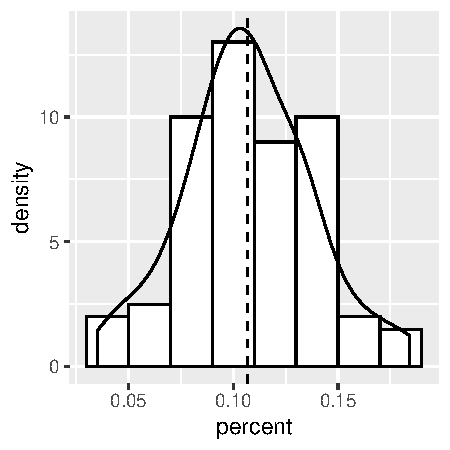
\includegraphics[width=\maxwidth]{figure/interval_data-1} 

}

\caption[Percentage of Damaged Printers per Trial (100 Visits)]{Percentage of Damaged Printers per Trial (100 Visits)}\label{fig:interval_data}
\end{figure}


\end{knitrout}

        \newpage
        @ \textit{For each of the 100 visits, make a 95\% confidence interval for the percentage of damaged printers you
        count.  How many of these confidence intervals contain the true percentage of $0.10$? Is this close to what you
        expected?}
        @@ We can create a function that logically indexes our data frame in order to determine which generated
        confidence intervals contain our true percentage, and then determine the length.

\begin{knitrout}
\definecolor{shadecolor}{rgb}{0.969, 0.969, 0.969}\color{fgcolor}\begin{kframe}
\begin{alltt}
         \hlstd{in_interval} \hlkwb{<-} \hlkwa{function}\hlstd{(}\hlkwc{m}\hlstd{,} \hlkwc{n}\hlstd{) \{}
             \hlstd{clower} \hlkwb{<-} \hlstd{m} \hlopt{-} \hlkwd{abs}\hlstd{(z} \hlopt{*} \hlkwd{sqrt}\hlstd{((m} \hlopt{*} \hlstd{(}\hlnum{1} \hlopt{-} \hlstd{m))} \hlopt{/} \hlstd{n))}
             \hlstd{cupper} \hlkwb{<-} \hlstd{m} \hlopt{+} \hlkwd{abs}\hlstd{(z} \hlopt{*} \hlkwd{sqrt}\hlstd{((m} \hlopt{*} \hlstd{(}\hlnum{1} \hlopt{-} \hlstd{m))} \hlopt{/} \hlstd{n))}
             \hlstd{(clower} \hlopt{<} \hlnum{0.10}\hlstd{)} \hlopt{&} \hlstd{(}\hlnum{0.10} \hlopt{<} \hlstd{cupper)}
         \hlstd{\}}
         \hlstd{count100} \hlkwb{<-} \hlkwd{length}\hlstd{(interval_data100}\hlopt{$}\hlstd{percent[}
                         \hlkwd{in_interval}\hlstd{(interval_data100}\hlopt{$}\hlstd{percent, n)])}
\end{alltt}
\end{kframe}
\end{knitrout}

        This results in $91$ intervals that contain the true percentage. We expected 95 of them, but this
        is close enough.\footnote{Note, this count is regenerated every time this paper is recompiled. If my above
        statement makes no sense, please forgive the grammatically insensitive random data generator.} Note, this goes
        back to the definition of a 95\% confidence interval as we can see that $91/100$ contained the
        true percentage. This is as it should be. Since the data is randomly generated however, we won't always get
        exactly 95 for this number.

        \newpage
        @ \textit{Repeat parts (4) and (5) with 500 visits and 1000 visits. What do you notice about your histogram?
        What theory are you observing? What do you notice about the number of confidence intervals that contain the true
        percentage?}
        @@ First, we establish our data using the {\ttfamily rbinom} command, and then we create a data frame with the
        given data. This data frame's first column is the number of damaged printers counted, and the second column is
        the percentage. Next we count how many confidence intervals generated using the sample percentage contain the
        true percentage.

\begin{knitrout}
\definecolor{shadecolor}{rgb}{0.969, 0.969, 0.969}\color{fgcolor}\begin{kframe}
\begin{alltt}
         \hlcom{# Establish Data}
         \hlstd{db500} \hlkwb{<-} \hlkwd{rbinom}\hlstd{(}\hlnum{500}\hlstd{, n,} \hlnum{0.10}\hlstd{)}
         \hlstd{db1000} \hlkwb{<-} \hlkwd{rbinom}\hlstd{(}\hlnum{1000}\hlstd{, n,} \hlnum{0.10}\hlstd{)}

         \hlcom{# Create Data Frames}
         \hlstd{interval_data500} \hlkwb{<-} \hlkwd{data.frame}\hlstd{(}\hlkwc{printers}\hlstd{=db500,} \hlkwc{percent}\hlstd{=db500}\hlopt{/}\hlstd{n)}
         \hlstd{interval_data1000} \hlkwb{<-} \hlkwd{data.frame}\hlstd{(}\hlkwc{printers}\hlstd{=db1000,} \hlkwc{percent}\hlstd{=db1000}\hlopt{/}\hlstd{n)}

         \hlcom{# Plot our distributions}
         \hlkwd{ggplot}\hlstd{(interval_data500,} \hlkwd{aes}\hlstd{(percent))} \hlopt{+}
                    \hlkwd{geom_histogram}\hlstd{(}\hlkwd{aes}\hlstd{(}\hlkwc{y}\hlstd{=..density..),} \hlkwc{binwidth}\hlstd{=}\hlnum{0.02}\hlstd{,}
                                   \hlkwc{color}\hlstd{=}\hlstr{'black'}\hlstd{,} \hlkwc{fill}\hlstd{=}\hlstr{'white'}\hlstd{)} \hlopt{+}
                    \hlkwd{geom_vline}\hlstd{(}\hlkwd{aes}\hlstd{(}\hlkwc{xintercept}\hlstd{=}\hlkwd{mean}\hlstd{(percent,} \hlkwc{na.rm}\hlstd{=T)),}
                               \hlkwc{color}\hlstd{=}\hlstr{"black"}\hlstd{,} \hlkwc{linetype}\hlstd{=}\hlstr{"dashed"}\hlstd{,} \hlkwc{size}\hlstd{=}\hlnum{0.5}\hlstd{)} \hlopt{+}
                    \hlkwd{geom_density}\hlstd{(}\hlkwc{alpha}\hlstd{=}\hlnum{0.2}\hlstd{)}

         \hlkwd{ggplot}\hlstd{(interval_data1000,} \hlkwd{aes}\hlstd{(percent))} \hlopt{+}
                    \hlkwd{geom_histogram}\hlstd{(}\hlkwd{aes}\hlstd{(}\hlkwc{y}\hlstd{=..density..),} \hlkwc{binwidth}\hlstd{=}\hlnum{0.02}\hlstd{,}
                                   \hlkwc{color}\hlstd{=}\hlstr{'black'}\hlstd{,} \hlkwc{fill}\hlstd{=}\hlstr{'white'}\hlstd{)} \hlopt{+}
                    \hlkwd{geom_vline}\hlstd{(}\hlkwd{aes}\hlstd{(}\hlkwc{xintercept}\hlstd{=}\hlkwd{mean}\hlstd{(percent,} \hlkwc{na.rm}\hlstd{=T)),}
                               \hlkwc{color}\hlstd{=}\hlstr{"black"}\hlstd{,} \hlkwc{linetype}\hlstd{=}\hlstr{"dashed"}\hlstd{,} \hlkwc{size}\hlstd{=}\hlnum{0.5}\hlstd{)} \hlopt{+}
                    \hlkwd{geom_density}\hlstd{(}\hlkwc{alpha}\hlstd{=}\hlnum{0.2}\hlstd{)}

         \hlcom{# Count instances of percentage within interval}
         \hlstd{count500} \hlkwb{<-} \hlkwd{length}\hlstd{(interval_data500}\hlopt{$}\hlstd{percent[}
                             \hlkwd{in_interval}\hlstd{(interval_data500}\hlopt{$}\hlstd{percent, n)])}
         \hlstd{count1000} \hlkwb{<-} \hlkwd{length}\hlstd{(interval_data1000}\hlopt{$}\hlstd{percent[}
                         \hlkwd{in_interval}\hlstd{(interval_data1000}\hlopt{$}\hlstd{percent, n)])}
\end{alltt}
\end{kframe}\begin{figure}[H]

{\centering \subfloat[500 Visits\label{fig:multivisits1}]{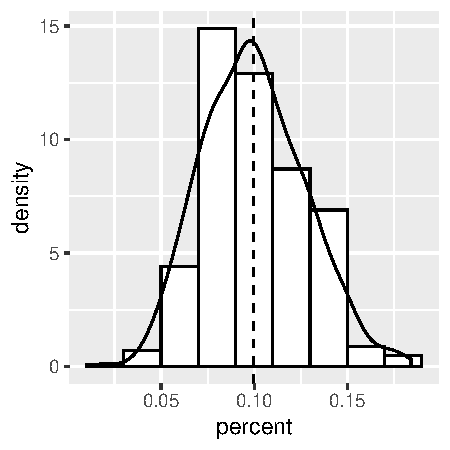
\includegraphics[width=0.45\textwidth]{figure/multivisits-1} }
\subfloat[1000 Visits\label{fig:multivisits2}]{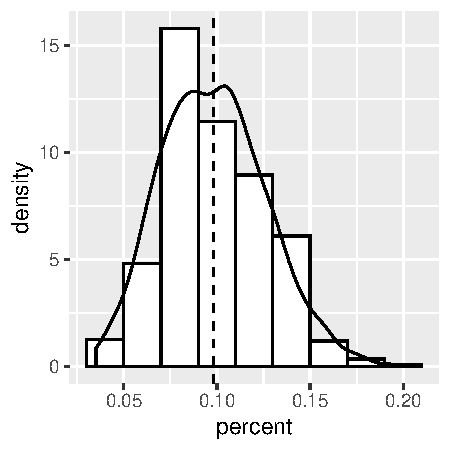
\includegraphics[width=0.45\textwidth]{figure/multivisits-2} }

}

\caption[Percentage of Damaged Printers per Trial]{Percentage of Damaged Printers per Trial}\label{fig:multivisits}
\end{figure}


\end{knitrout}

        In Figure~\ref{fig:multivisits1} we see that not only is the histogram density becoming more and more smooth,
        but that the Central Limit Theorem is holding. The Central Limit Theorem roughly states that expected value of
        our estimators will approach the true value as the amount of data grows. If we examine our count, we see that it
        is $0.942$, which is also close to 95\%\footnote{Ibid.}. We can now move to 1000 visits.
        \newline

        In Figure~\ref{fig:multivisits2} we see that our histogram is a very accurate model of the situation with
        again, the Central Limit Theorem as to the reason why. If we now examine our count, we see that it is
        $0.934$, which is also close to 95\%.\footnote{Ibid.}

        \newpage
        @ \textit{Make a histogram of the p-values for the 1000 visits, testing if the manufacturer's claim is true.
        What does the distribution of your p-values look like?}
        @@ In this case we assume our null hypothesis is that the percent of damaged printers is 10\%. We can examine
        each generated element to determine whether or not our null hypothesis is valid. In this case our test is
        two-tailed, as the data could be either too high, or too low, and we need to just test that our sample
        percentage is not equal to our true percentage. In other words, we need to test

        \[
            H_0 \neq H_a
        \]

\begin{knitrout}
\definecolor{shadecolor}{rgb}{0.969, 0.969, 0.969}\color{fgcolor}\begin{kframe}
\begin{alltt}
         \hlstd{z_test} \hlkwb{<-} \hlstd{(p_hat} \hlopt{-} \hlstd{interval_data1000}\hlopt{$}\hlstd{percent)}\hlopt{/}\hlstd{(}\hlkwd{sqrt}\hlstd{((}
                  \hlstd{interval_data1000}\hlopt{$}\hlstd{percent} \hlopt{*}
                  \hlstd{(}\hlnum{1} \hlopt{-} \hlstd{interval_data1000}\hlopt{$}\hlstd{percent))}\hlopt{/}\hlstd{n))}
         \hlstd{interval_data1000p} \hlkwb{<-} \hlkwd{data.frame}\hlstd{(}\hlkwc{printers}\hlstd{=interval_data1000}\hlopt{$}\hlstd{printers,}
                                     \hlkwc{percent}\hlstd{=interval_data1000}\hlopt{$}\hlstd{percent,}
                                     \hlkwc{pvalues}\hlstd{=}\hlnum{2} \hlopt{*} \hlstd{(}\hlnum{1} \hlopt{-} \hlkwd{pnorm}\hlstd{(}\hlkwd{abs}\hlstd{(z_test))))}
         \hlkwd{ggplot}\hlstd{(interval_data1000p,} \hlkwd{aes}\hlstd{(pvalues))} \hlopt{+}
                    \hlkwd{scale_x_continuous}\hlstd{(}\hlkwc{limits} \hlstd{=} \hlkwd{c}\hlstd{(}\hlnum{0}\hlstd{,} \hlnum{1}\hlstd{))} \hlopt{+}
                    \hlkwd{geom_histogram}\hlstd{(}\hlkwd{aes}\hlstd{(}\hlkwc{y}\hlstd{=..density..),} \hlkwc{binwidth}\hlstd{=}\hlnum{0.1}\hlstd{,}
                                   \hlkwc{color}\hlstd{=}\hlstr{'black'}\hlstd{,} \hlkwc{fill}\hlstd{=}\hlstr{'white'}\hlstd{)} \hlopt{+}
                    \hlkwd{geom_vline}\hlstd{(}\hlkwd{aes}\hlstd{(}\hlkwc{xintercept}\hlstd{=}\hlnum{0.1}\hlstd{),}
                               \hlkwc{color}\hlstd{=}\hlstr{"red"}\hlstd{,} \hlkwc{linetype}\hlstd{=}\hlstr{"solid"}\hlstd{,} \hlkwc{size}\hlstd{=}\hlnum{0.5}\hlstd{)} \hlopt{+}
                    \hlkwd{geom_vline}\hlstd{(}\hlkwd{aes}\hlstd{(}\hlkwc{xintercept}\hlstd{=}\hlnum{0.05}\hlstd{),}
                               \hlkwc{color}\hlstd{=}\hlstr{"red"}\hlstd{,} \hlkwc{linetype}\hlstd{=}\hlstr{"solid"}\hlstd{,} \hlkwc{size}\hlstd{=}\hlnum{0.5}\hlstd{)} \hlopt{+}
                    \hlkwd{geom_vline}\hlstd{(}\hlkwd{aes}\hlstd{(}\hlkwc{xintercept}\hlstd{=}\hlnum{0.01}\hlstd{),}
                               \hlkwc{color}\hlstd{=}\hlstr{"red"}\hlstd{,} \hlkwc{linetype}\hlstd{=}\hlstr{"solid"}\hlstd{,} \hlkwc{size}\hlstd{=}\hlnum{0.5}\hlstd{)}
\end{alltt}


{\ttfamily\noindent\color{warningcolor}{\#\# Warning: Removed 2 rows containing missing values (geom\_bar).}}\end{kframe}\begin{figure}[H]

{\centering 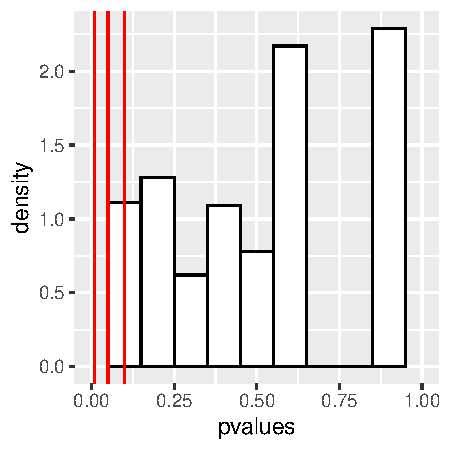
\includegraphics[width=\maxwidth]{figure/pvalues-1} 

}

\caption[Distribution of our $P$-Values]{Distribution of our $P$-Values}\label{fig:pvalues}
\end{figure}


\end{knitrout}

        In Figure~\ref{fig:pvalues} we mark $p=0.01, p=0.05$, and $p=0.1$ to indicate rejection zones. These $p$-values
        are distributed fairly uniformly, and as a result this graph does not tell us much about whther or not our null
        hypothesis is valid; all it tells us is that the null \textit{might} be invalid. Based on our other parts we've
        previously calculated however, we know that the manufacturer's claim is most likely true.

        \newpage
        @ \textit{Repeat parts (4)-(7), but simulate the number of damaged printers assuming a $Bin(n, 0.25)$
        distribution. As the inspector, you do not know if the manufacturer is telling the truth, but you are a great
        statistician who knows how to analyze data properly. After examining your histogram, the confidence intervals, and
        the p-values, what would you conclude about the veracity of the manufacturer's claim? And, more importantly,
        Why?}\newline
        @@ First we can simulate the data using the new distribution in the same manner as part (4). Please reference
        Figure~\ref{fig:interval_data_new}. Note the mean-line remains, but is markedly different from before due to the
        new distribution.

\begin{knitrout}
\definecolor{shadecolor}{rgb}{0.969, 0.969, 0.969}\color{fgcolor}\begin{kframe}
\begin{alltt}
         \hlstd{db100_new} \hlkwb{<-} \hlkwd{rbinom}\hlstd{(}\hlnum{100}\hlstd{, n,} \hlnum{0.25}\hlstd{)}
         \hlstd{interval_data100_new} \hlkwb{<-} \hlkwd{data.frame}\hlstd{(}\hlkwc{printers}\hlstd{=db100_new,} \hlkwc{percent}\hlstd{=db100_new}\hlopt{/}\hlstd{n)}
         \hlkwd{ggplot}\hlstd{(interval_data100_new,} \hlkwd{aes}\hlstd{(percent))} \hlopt{+}
                    \hlkwd{geom_histogram}\hlstd{(}\hlkwd{aes}\hlstd{(}\hlkwc{y}\hlstd{=..density..),} \hlkwc{binwidth}\hlstd{=}\hlnum{0.02}\hlstd{,}
                                   \hlkwc{color}\hlstd{=}\hlstr{'black'}\hlstd{,} \hlkwc{fill}\hlstd{=}\hlstr{'white'}\hlstd{)} \hlopt{+}
                    \hlkwd{geom_vline}\hlstd{(}\hlkwd{aes}\hlstd{(}\hlkwc{xintercept}\hlstd{=}\hlkwd{mean}\hlstd{(percent,} \hlkwc{na.rm}\hlstd{=T)),}
                               \hlkwc{color}\hlstd{=}\hlstr{"black"}\hlstd{,} \hlkwc{linetype}\hlstd{=}\hlstr{"dashed"}\hlstd{,} \hlkwc{size}\hlstd{=}\hlnum{0.5}\hlstd{)} \hlopt{+}
                    \hlkwd{geom_density}\hlstd{(}\hlkwc{alpha}\hlstd{=}\hlnum{0.2}\hlstd{)}
\end{alltt}
\end{kframe}\begin{figure}[H]

{\centering 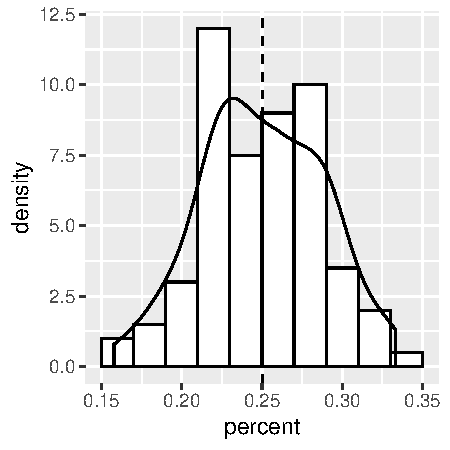
\includegraphics[width=\maxwidth]{figure/interval_data_new-1} 

}

\caption[Percentage of Damaged Printers per Trial (100 Visits)]{Percentage of Damaged Printers per Trial (100 Visits)}\label{fig:interval_data_new}
\end{figure}


\end{knitrout}

        Now we can re-use our function from above to determine how many sample percentages are within the sample's
        calculated confidence interval.

\begin{knitrout}
\definecolor{shadecolor}{rgb}{0.969, 0.969, 0.969}\color{fgcolor}\begin{kframe}
\begin{alltt}
         \hlstd{count100_new} \hlkwb{<-} \hlkwd{length}\hlstd{(interval_data100_new}\hlopt{$}\hlstd{percent[}
                         \hlkwd{in_interval}\hlstd{(interval_data100_new}\hlopt{$}\hlstd{percent, n)])}
\end{alltt}
\end{kframe}
\end{knitrout}

        And we see that the percent of confidence intervals that contain our true percentage under the null hypothesis
        is $0.02$. We can now extend the experiment using 500 and 1000 visits as before.

\begin{knitrout}
\definecolor{shadecolor}{rgb}{0.969, 0.969, 0.969}\color{fgcolor}\begin{kframe}
\begin{alltt}
         \hlcom{# Establish Data}
         \hlstd{db500_new} \hlkwb{<-} \hlkwd{rbinom}\hlstd{(}\hlnum{500}\hlstd{, n,} \hlnum{0.25}\hlstd{)}
         \hlstd{db1000_new} \hlkwb{<-} \hlkwd{rbinom}\hlstd{(}\hlnum{1000}\hlstd{, n,} \hlnum{0.25}\hlstd{)}

         \hlcom{# Create Data Frames}
         \hlstd{interval_data500_new} \hlkwb{<-} \hlkwd{data.frame}\hlstd{(}\hlkwc{printers}\hlstd{=db500_new,}
                                            \hlkwc{percent}\hlstd{=db500_new}\hlopt{/}\hlstd{n)}
         \hlstd{interval_data1000_new} \hlkwb{<-} \hlkwd{data.frame}\hlstd{(}\hlkwc{printers}\hlstd{=db1000_new,}
                                             \hlkwc{percent}\hlstd{=db1000_new}\hlopt{/}\hlstd{n)}

         \hlcom{# Plot our distributions}
         \hlkwd{ggplot}\hlstd{(interval_data500_new,} \hlkwd{aes}\hlstd{(percent))} \hlopt{+}
                    \hlkwd{geom_histogram}\hlstd{(}\hlkwd{aes}\hlstd{(}\hlkwc{y}\hlstd{=..density..),} \hlkwc{binwidth}\hlstd{=}\hlnum{0.02}\hlstd{,}
                                   \hlkwc{color}\hlstd{=}\hlstr{'black'}\hlstd{,} \hlkwc{fill}\hlstd{=}\hlstr{'white'}\hlstd{)} \hlopt{+}
                    \hlkwd{geom_vline}\hlstd{(}\hlkwd{aes}\hlstd{(}\hlkwc{xintercept}\hlstd{=}\hlkwd{mean}\hlstd{(percent,} \hlkwc{na.rm}\hlstd{=T)),}
                               \hlkwc{color}\hlstd{=}\hlstr{"black"}\hlstd{,} \hlkwc{linetype}\hlstd{=}\hlstr{"dashed"}\hlstd{,} \hlkwc{size}\hlstd{=}\hlnum{0.5}\hlstd{)} \hlopt{+}
                    \hlkwd{geom_density}\hlstd{(}\hlkwc{alpha}\hlstd{=}\hlnum{0.2}\hlstd{)}

         \hlkwd{ggplot}\hlstd{(interval_data1000_new,} \hlkwd{aes}\hlstd{(percent))} \hlopt{+}
                    \hlkwd{geom_histogram}\hlstd{(}\hlkwd{aes}\hlstd{(}\hlkwc{y}\hlstd{=..density..),} \hlkwc{binwidth}\hlstd{=}\hlnum{0.02}\hlstd{,}
                                   \hlkwc{color}\hlstd{=}\hlstr{'black'}\hlstd{,} \hlkwc{fill}\hlstd{=}\hlstr{'white'}\hlstd{)} \hlopt{+}
                    \hlkwd{geom_vline}\hlstd{(}\hlkwd{aes}\hlstd{(}\hlkwc{xintercept}\hlstd{=}\hlkwd{mean}\hlstd{(percent,} \hlkwc{na.rm}\hlstd{=T)),}
                               \hlkwc{color}\hlstd{=}\hlstr{"black"}\hlstd{,} \hlkwc{linetype}\hlstd{=}\hlstr{"dashed"}\hlstd{,} \hlkwc{size}\hlstd{=}\hlnum{0.5}\hlstd{)} \hlopt{+}
                    \hlkwd{geom_density}\hlstd{(}\hlkwc{alpha}\hlstd{=}\hlnum{0.2}\hlstd{)}

         \hlcom{# Count instances of percentage within interval}
         \hlstd{count500_new} \hlkwb{<-} \hlkwd{length}\hlstd{(interval_data500_new}\hlopt{$}\hlstd{percent[}
                             \hlkwd{in_interval}\hlstd{(interval_data500_new}\hlopt{$}\hlstd{percent, n)])}
         \hlstd{count1000_new} \hlkwb{<-} \hlkwd{length}\hlstd{(interval_data1000_new}\hlopt{$}\hlstd{percent[}
                         \hlkwd{in_interval}\hlstd{(interval_data1000_new}\hlopt{$}\hlstd{percent, n)])}
\end{alltt}
\end{kframe}\begin{figure}[H]

{\centering \subfloat[500 Visits\label{fig:multivisits_new1}]{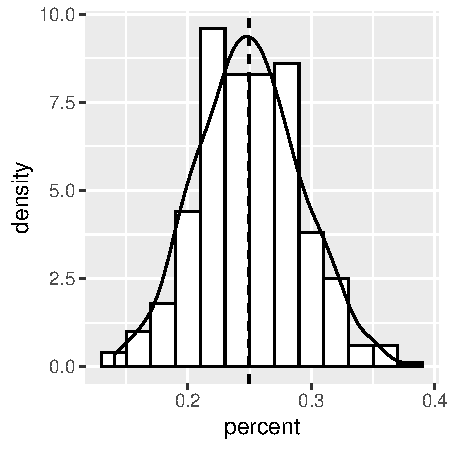
\includegraphics[width=0.45\textwidth]{figure/multivisits_new-1} }
\subfloat[1000 Visits\label{fig:multivisits_new2}]{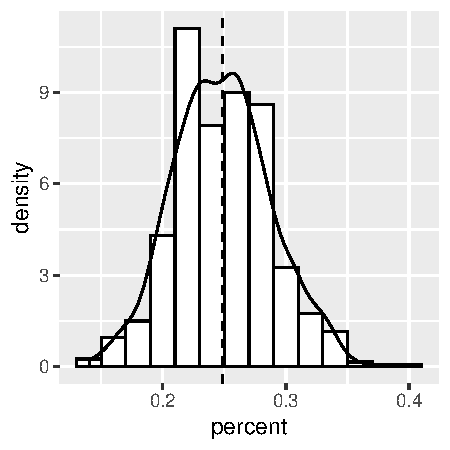
\includegraphics[width=0.45\textwidth]{figure/multivisits_new-2} }

}

\caption[Percentage of Damaged Printers per Trial]{Percentage of Damaged Printers per Trial}\label{fig:multivisits_new}
\end{figure}


\end{knitrout}

        Repeating with 500 and 1000 visits respectively, we obtain $0.028$ and
        $0.024$ percent of sample confidence intervals that contain our true percentage of
        $0.10$.\newline

        We can now look at the $p$-values.

\begin{knitrout}
\definecolor{shadecolor}{rgb}{0.969, 0.969, 0.969}\color{fgcolor}\begin{kframe}
\begin{alltt}
         \hlstd{z_test} \hlkwb{<-} \hlstd{(p_hat} \hlopt{-} \hlstd{interval_data1000_new}\hlopt{$}\hlstd{percent)}\hlopt{/}\hlstd{(}\hlkwd{sqrt}\hlstd{((}
                  \hlstd{interval_data1000_new}\hlopt{$}\hlstd{percent} \hlopt{*}
                  \hlstd{(}\hlnum{1} \hlopt{-} \hlstd{interval_data1000_new}\hlopt{$}\hlstd{percent))}\hlopt{/}\hlstd{n))}
         \hlstd{interval_data1000p_new} \hlkwb{<-} \hlkwd{data.frame}\hlstd{(}
                                 \hlkwc{printers}\hlstd{=interval_data1000_new}\hlopt{$}\hlstd{printers,}
                                 \hlkwc{percent}\hlstd{=interval_data1000_new}\hlopt{$}\hlstd{percent,}
                                 \hlkwc{pvalues}\hlstd{=}\hlnum{2} \hlopt{*} \hlstd{(}\hlnum{1} \hlopt{-} \hlkwd{pnorm}\hlstd{(}\hlkwd{abs}\hlstd{(z_test))))}
         \hlkwd{ggplot}\hlstd{(interval_data1000p_new,} \hlkwd{aes}\hlstd{(pvalues))} \hlopt{+}
                    \hlkwd{scale_x_continuous}\hlstd{(}\hlkwc{limits} \hlstd{=} \hlkwd{c}\hlstd{(}\hlnum{0}\hlstd{,} \hlnum{0.11}\hlstd{))} \hlopt{+}
                    \hlkwd{geom_histogram}\hlstd{(}\hlkwd{aes}\hlstd{(}\hlkwc{y}\hlstd{=..density..),} \hlkwc{binwidth}\hlstd{=}\hlnum{0.02}\hlstd{,}
                                   \hlkwc{color}\hlstd{=}\hlstr{'black'}\hlstd{,} \hlkwc{fill}\hlstd{=}\hlstr{'white'}\hlstd{)} \hlopt{+}
                    \hlkwd{geom_vline}\hlstd{(}\hlkwd{aes}\hlstd{(}\hlkwc{xintercept}\hlstd{=}\hlnum{0.1}\hlstd{),}
                               \hlkwc{color}\hlstd{=}\hlstr{"red"}\hlstd{,} \hlkwc{linetype}\hlstd{=}\hlstr{"solid"}\hlstd{,} \hlkwc{size}\hlstd{=}\hlnum{0.5}\hlstd{)} \hlopt{+}
                    \hlkwd{geom_vline}\hlstd{(}\hlkwd{aes}\hlstd{(}\hlkwc{xintercept}\hlstd{=}\hlnum{0.05}\hlstd{),}
                               \hlkwc{color}\hlstd{=}\hlstr{"red"}\hlstd{,} \hlkwc{linetype}\hlstd{=}\hlstr{"solid"}\hlstd{,} \hlkwc{size}\hlstd{=}\hlnum{0.5}\hlstd{)} \hlopt{+}
                    \hlkwd{geom_vline}\hlstd{(}\hlkwd{aes}\hlstd{(}\hlkwc{xintercept}\hlstd{=}\hlnum{0.01}\hlstd{),}
                               \hlkwc{color}\hlstd{=}\hlstr{"red"}\hlstd{,} \hlkwc{linetype}\hlstd{=}\hlstr{"solid"}\hlstd{,} \hlkwc{size}\hlstd{=}\hlnum{0.5}\hlstd{)}
\end{alltt}


{\ttfamily\noindent\color{warningcolor}{\#\# Warning: Removed 5 rows containing non-finite values (stat\_bin).}}

{\ttfamily\noindent\color{warningcolor}{\#\# Warning: Removed 1 rows containing missing values (geom\_bar).}}\end{kframe}\begin{figure}[H]

{\centering 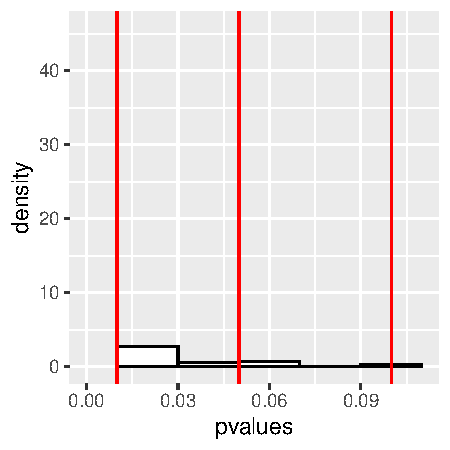
\includegraphics[width=\maxwidth]{figure/pvalues_new-1} 

}

\caption[Distribution of our $P$-Values]{Distribution of our $P$-Values}\label{fig:pvalues_new}
\end{figure}


\end{knitrout}

        After all the analysis is finished we can conclude that the printer manufacturer is incorrect in assuming that
        only 10\% of their printers are damaged. This conclusion is established from several different points. First, we
        can see just by plotting a histogram of the data that the average percent of damaged printers is about 25\%,
        which is a huge mark against the null hypothesis that our percentage is equal to 0.10.\newline

        Second, if we take a look at how many of our calculated confidence intervals contain our true mean, we see that
        this number is effectively zero, meaning that by definition we no longer have a 95\% confidence interval
        established, and something is incorrect.\newline

        Lastly, by examining our $p$-values we see that almost every single value is less than $0.10$, and most are
        below $0.01$, which idicates a very strong presumption against our null hypothesis.\newline

        Based on all the evidence we should reject our null hypothesis in favor of something else. Based on the
        experimental data it would not be incorrect to assume a contending null hypothesis to be $0.25$, which is indeed
        correct.

    \end{easylist}

\end{document}
